\chapter{系统总体设计}
\section{系统总体需求分析}
本小节主要分析了Rails消息总线项目的具体需求。本项目由三个子项目构成,Rails消息总线子项目用于提供从Rails服务器到浏览器的基础服务技术;Auto-Reload技术主要用于开发模式时自动检测源代码更改事件并通知浏览器进行刷新动作;而Backend Instrumentation技术则是通过在后台采集性能数据,并将其反馈到前端的技术。

\subsection{Rails消息总线需求分析}
Rails消息总线提供了一套机制,使得服务器能够实时地推送任意数据到浏览器客户端。本文从两个层面上实现了Rails消息总线技术,这两个层面抽象程度、易用性以及灵活性各不相同,适应于不同的应用场景。针对这两个层面,Rails消息总线技术提供了两套接口(模式)。 这两套接口中,抽象程度较低、更为灵活的是Raw Streaming Mode,使用这套接口,服务器可以发送任意格式的数据,HTTP报文的报头和内容完全由服务器定制而不受Rails框架限制。另一套接口是SSE Mode,该套接口抽象程度较高,使用更为简单。SSE Mode即Server Sent Events技术的Rails实现版本,Rails消息总线技术实现了较为完整的SSE技术规范,对于规范中大部分内容(特别是开发环境中最常使用的特性)都予以了支持。

对于Raw Streaming模式,Rails消息总线技术允许程序获取服务器和浏览器连接的原始套接字对象。并且允许开发者直接向该套接字读写数据,并且写入的数据将被即刻传输至浏览器,从而实现了实时数据推送。为了使得服务器能够推送数据,首先需要浏览器主动连接到Rails服务器上以获取数据。该过程需要通过浏览器向Rails服务器发送一个传统的HTTP连接请求来完成,因此在服务器端,开发者必须首先定义一个入口Controller和相应的action。当入口Controller和action定义好,并且在Rails项目的route.rb文件中注册完成之后,浏览器可以通过地址“http://server\_addr/controller/action”连接上Rails服务器。此时由于该路径已在route.rb中注册成功,Rails会将该请求路由到相应的Controller及其action上的代码处。此时,Rails开发者可以通过在相应的action中获取response对象,通过向数据流response.stream写入数据,可以实现超浏览器发送实时数据。代码\ref{raw-streaming-demo}展示了如何使用该接口:

\begin{lstlisting}[caption={Raw Streaming Mode使用示例}, label=raw-streaming-demo]
class MyController < ActionController::Base
  include ActionController::Live

  def stream
    response.headers['Content-Type'] = 'text/event-stream'
    100.times {
      response.stream.write "hello world\n"
      sleep 1
    }
    response.stream.close
  end
end
\end{lstlisting}

代码\ref{raw-streaming-demo}首先定义了一个Controller和action用于接收浏览器的请求。此时浏览器可以通过地址"http://server\_addr/my/stream"地址来访问服务器实时数据推送服务。当浏览器请求被Rails服务器接收后,ActionController\#Stream则会被调用,以响应浏览器得请求。

为了使用Rails实时消息推送机制,代码\ref{raw-streaming-demo}通过include ActionController::Live语句将ActionController::Live模块激活,从而启用了消息推送机制。这之后,开发这可以通过response.stream来向客户端发送任意数据。当然,开发者亦能够通过response.headers来设置响应HTTP报文得报头内容,从而更精细化地控制消息。这里值得指出的是,开发者只能够在response状态变成提交之前设置HTTP报头,否则消息总线系统将抛出一个异常。response状态编程提交的时机,便是开发者第一次调用response.stream.write或者response.stream.close的时候。如果开发者调用这两个接口任意一个,则response状态变为已提交,此时则将不能够设置HTTP报头内容。

最后,如果客户端没有显式地断开连接,服务器在停止服务之前必须显式地调用response.stream.close接口以关闭数据流。否则将会照成和客户端之间的连接不能被中断,系统资源难以回收,从而影响到服务器系统执行效率。

Rails消息总线技术提供的另一套接口则是基于标准的SSE规范的。该接口的实现,一则是为了提供一个抽象程度较高、十分易用的接口给Rails开发者,二则是为了是Rails能够支持HTML5新规范,特别是对于支持HTML5规范中SSE的浏览器(HTML5兼容浏览器)提供支持。使用该套接口,Rails会自动生成兼容的SSE消息格式,同浏览器交换元数据,并且实现断线重连等机制。但是对上,本技术向Rails开发者隐藏了此类复杂机制,对于其来说,Rails消息总线机制提供了一个稳定的、安全的、健壮的通信机制,使得其能够实时的向浏览器发送SSE兼容消息。

SSE接口同样提供了两种模式,一种是Controller Level SSE,另一种则是Client Level SSE。对于前一种模式来说,Rails不区分连接到自己的不同客户端。当开发者发送SSE消息至客户端后,所有当前连接的客户端均会收到该条消息。使用Controller Level SSE,开发者不需要遍历客户端列表,并逐一发送SSE消息,这对于某些全局通用消息的发送场合能够大大提高效率。但是,由于Controller Level SSE对客户端不做区分,这使得系统无法针对不同客户端推送不同消息。而针对不同客户端推送不同消息在某些应用场景下是十分关键和重要的(例如微博消息推送、论坛和网站的即时消息等)。针对这类应用场景,Rails消息总线技术提供了Client Level SSE予以解决。通过使用Client Level SSE,开发者将在不同的线程中响应浏览器请求并发送即时消息。并且,开发者同时能够获取当前回话相关的变量,例如cookies、HTTP请求报头、HTTP请求变量等等和具体客户端相关联的数据。据此,开发者能够实现针对不同的客户端,推送不同的消息。

对于Controller Level SSE,可以通过下面的代码来使用之:

\begin{lstlisting}[caption={Controller Level SSE示例}, label=cls-demo]
# SSE entry controller
class MyController < ActionController::Base
  include ActionController::Live
  include ActionController::ServerSentEvents
  extend ActionController::ServerSentEvents::ClassMethods
end

# when we want to send an event
@sse = ServerSentEvent.new "this is data"
MyController.send_sse @sse

# send an event through another interface
MyController.send_sse_hash :data => "this is also data"
\end{lstlisting}

在代码\ref{cls-demo}中,为了定义一个Controller Level SSE的入口Controller和action,代码分别include了ActionController::Live和ActionController::ServerSentEvents两个模块,并且extend了ActionController::ServerSentEvents::ClassMethods模块。

通过上述三行代码,使得MyController成为了Controller Level SSE的入口。这时候一个叫做sse\_source的action将被自动定义,开发者需要将该action注册到route.rb文件中,从而使得Rails路由系统能够找到是sse\_source action。这时候,浏览器通过访问“http://server\_addr/my/sse\_source",则可以接收相应的SSE消息。

在代码\ref{cls-demo}同时展示了如何发送一条消息至客户端。可以看到,使用MyController\#send\_sse接口,需要首先生成一个ServerSentEvent对象,并将其作为参数发送;而若使用MyController\#send\_sse\_hash接口,则可以直接以一个哈希表为参数,此时哈希表中:data键所对应的数据则是待发送数据。值得指出的是,MyController\#send\_sse以及MyController\#send\_sse\_hash可以在任何线程中执行。其执行结果是,所有连接到“http://server\_addr/my/sse\_source”的浏览器都会接受到该SSE全局消息。

Rails消息总线为SSE提供的另一个接口便是Client Level SSE。代码\ref{cls2-demo}展示了如何使用该技术:

\begin{lstlisting}[caption={Client Level SSE示例}, label=cls2-demo]
class MySSE < ActionController::Base
  include ActionController::Live
  include ActionController::ServerSentEvents

  def event
    start_serve do |sse_client|
      # we can access some session variables here
      sse_client.send_sse sse
      sse_client.send_sse_hash :data => "david"
    end
  end
end
\end{lstlisting}

代码\ref{cls2-demo}首先定义了一个Controller及一个action,并手动在route.rb文件中注册相应的路由策略。这样,客户端浏览器便可以通过地址“http://server\_addr/my/event”连接到该数据源服务器上。在event方法内,只有一个start\_serve调用,该函数的执行将使得服务器一直持有对客户端浏览器之间的原始套接字,并且通过调用关联的回调方法向原始套接字中写入数据。可以看到,在调用start\_serve的同时,代码\ref{cls2-demo}传入了一个Block对象。该对象作为一个回调函数,用于处理实际向客户端原始套接字写入数据的任务。该回调函数拥有一个参数,该参数是一个sse\_client对象,借以该对象的send\_sse\_hash和send\_sse两个接口,开发者可以直接向客户端发送SSE消息。

值得指出的是,Client Level SSE和Controller Level SSE在消息发送接口上十分接近。前者通过回调函数的参数获取一个sse\_client对象,并通过向该对象的send\_sse\_hash和send\_sse两个接口从而实现向客户端浏览器发送SSE消息的功能;而后者则是通过在任意时刻通过Controller的两个类方法send\_sse\_hash和send\_sse,来实现向全部连接到该数据源的客户端浏览器发送SSE消息的功能。另外,可以看到,Client Level SSE是不需要extend模块ActionController::ServerSentEvents::ClassMethods的。这是因为Client Level SSE模式需要开发者自行定义和编写数据源入口action的代码。

\subsection{Auto-Reload需求分析}
Auto-Reload是针对于Rails开发者的辅助技术,它实现了自动检测Rails后台源码更改并通知浏览器即时刷新的功能。在现代的网站开发过程中,一个基本网站的构建依赖于众多技术的支持,这产生了对数量庞大的源代码文件的依赖。这些代码文件既包括网站后台逻辑的代码,也包括网页前台的HTML定义文件,层叠样式表CSS文件,前端逻辑的JavaScript文件等等。对这些文件当中的任何一个部分进行更改对整个网站来说,都是牵一发而动全身的。

传统上,由于对这些源文件更改的效果,需要网站开发者重新编译并且部署网站,方能够看到改动后的效果。这需要开发者投入大量的精力和时间,对于正在专注于代码逻辑编写的开发者来说,这一系列繁琐的过程势必使得其开发效率大打折扣。在Rails中,为了极大的提高Rails开发者的生产效率,本文引入了一项新的称之为Auto-Reload的技术。该技术充分利用了Ruby这门动态脚本语言的特性,结合Rails框架自身的灵活性,实现了后台代码一旦改动,前端调试页面立刻刷新而不需要开发者手动干预这么一个功能。

由于Ruby是一门非编译型的动态脚本语言,这使得对后台代码的更改能够立刻体现到程序逻辑之上而不需要重新经历一遍传统开发语言所必须经历的编译、链接、部署等过程。这为Auto-Reload的实现客观上创造了可能性。但是,为了引入改动代码所带来的变化,我们依旧需要浏览器重新向后台服务器请求新的页面。于是,Auto-Reload便承担了这项工作。Auto-Reload自动监测Rails工程文件夹下所有的文件系统消息,并筛选处一切对可能影响网站逻辑、外观的文件(.rb文件,.css文件,.js文件,.html文件等等)的变动消息。一旦发觉此种文件被改动了,则立刻通过Rails消息总线通知客户端浏览器文件的变动,并告知其立刻刷新。与此同时,在客户端浏览器中,本技术通过一个JavaScript脚本向后台Rails服务器订阅一个关于文件变动消息的SSE消息源。一旦JavaScript脚本接受到文件变动消息,则指导浏览器进行网页刷新动作,重新发送HTTP请求,载入新的网页页面、并重新渲染改动后网页。

Auto-Reload对外实现了良好的接口,只需要开发者在Rails工程的Gemfile里指出想要使用auto-reload即可。下面的代码演示了如何使用Auto-Relaod技术

\begin{lstlisting}[caption={启用Auto-Realod技术}, label=auto-reload-demo]
source 'https://rubygems.org'

gem 'rack', path: '/Users/david/work_place/projects/rack'
gem 'rails',     path: '/Users/david/work_place/projects/rails'
gem 'arel',      github: 'rails/arel'
gem 'activerecord-deprecated_finders', github: 'rails/activerecord-deprecated_finders'
gem 'debugger'
gem 'sqlite3'
gem 'puma'

# To enable Auto-Reload feature
gem 'autorelaod', path: '/Users/david/work_place/projects/auto_reload'

# Gems used only for assets and not required
# in production environments by default.
group :assets do
  gem 'sprockets-rails', github: 'rails/sprockets-rails'
  gem 'sass-rails',   github: 'rails/sass-rails'
  gem 'coffee-rails', github: 'rails/coffee-rails'
  gem 'uglifier', '>= 1.0.3'
end

gem 'jquery-rails', github: 'rails/jquery-rails'

# Deploy with Capistrano
# gem 'capistrano', group: :development

# To use debugger
gem 'debugger', group: [:development, :test]
\end{lstlisting}

可以看到,Auto-Reload技术的使用十分简单和直观。在代码\ref{auto-reload-demo}的12行中,通过一个gem语句指明了开发者想要使用Auto-Reload技术的意图,从而使得Auto—Reload作为一个Gem在服务器启动阶段被Rails载入到内存中。这之后,开发者需要在网页中手动加入JAvaScript代码订阅SSE消息并在接收到文件变动消息时指导浏览器刷新。

\subsection{Backend Instrumentation需求分析}

Backend Instrumentation则是另外一项开发者支持技术。它是用于实现Rails框架的网页式后台管理终端的一个主要技术之一。Backend Instrumentation支持实时的对Rails服务器进行性能评估和测试,并对评估和测试结果进行实时的计算和统计。通过收集和统计这些数据,能够使得开发者更为清晰地了解到Rails服务器后台目前的运行状态。这对于传统的后台开发来说并不是新的技术,对于传统的网页开发来说,却很难实现一个基于网页的后台管理和调试中断系统。Backend Instrumentation技术则在后台收集到数据之后,通过Rails消息总线技术,将数据传送到前端浏览器的消息订阅者处,从而实现了实时性能数据的推送,为Rails服务器前台网页式管理终端的实现提供了基础。

启用Backend Instrumentation技术依旧十分简单。首先需要确保本地机器上安装好了名为backendinstrument的Gem,然后开发者需要在Rails项目的Gemfile中指定使用该Gem,如下代码所示:

\begin{lstlisting}[caption={启用Auto-Realod技术}, label=backend-demo]
source 'https://rubygems.org'

gem 'rack', path: '/Users/david/work_place/projects/rack'
gem 'rails',     path: '/Users/david/work_place/projects/rails'
gem 'arel',      github: 'rails/arel'
gem 'activerecord-deprecated_finders', github: 'rails/activerecord-deprecated_finders'
gem 'debugger'
gem 'sqlite3'
gem 'puma'

# Enable Backend Instrumentation feature to get realtime performance data
gem 'backendinstrument', path: '/Users/david/work_place/projects/backend_instrument', group: [:deployment]
\end{lstlisting}

代码\ref{backend-demo}的12行指明了如何启用Backend Instrumentation技术。通过在Gemfile里使用gem语句,开发者告知Rails框架在启动时载入backendinstrument Gem,从而使得Backend Instrumentation技术的代码被载入至内存。这样,在程序运行期间,Backend Instrumentation技术将持续收集Rials服务器的性能数据,并将其推送至所有的前台消息订阅者处。值得指出的是,这里使用一个group子句,指明了Backend Instrumentation技术仅仅在网站部署时有效。这样设计是符合一般常识的,因为开发者一般仅希望在网站正式运行时才通过Backend Instrumentation技术抓去后台运行性能数据,从而实现远程监控和管理。

\section{解决方案概要}
本小节基于上一小节对Rails消息总线技术需求的具体分析,从宏观上给出了一个解决方案概览,并且在后续子小节中对该宏观概览图的子部分的解决方案亦进行了概要性的描述。本节对系统整体解决方案的描述,将作为本文详细技术细节设计的标准,并指导后续工作的完成。

\subsection{系统总体解决方案}
Rails消息总线技术是一门允许网页服务器向浏览器客户端发送实时数据的技术,该技术作为Rails技术中的一门新的基础性技术,将始终贯穿于Rails其他部件的发展之中,亦和Rails开发人员之间关系密切。由于Rails消息总线技术的基础性,将使得该技术对任意Rails组件可见,它提供了简洁并且强大的API供上层逻辑调用。

为了阐述清楚Rails消息总线技术的大体结构,图\ref{fig-infra}中展示了Rails消息总线技术的宏观架构:

\begin{figure}[h]
\centering
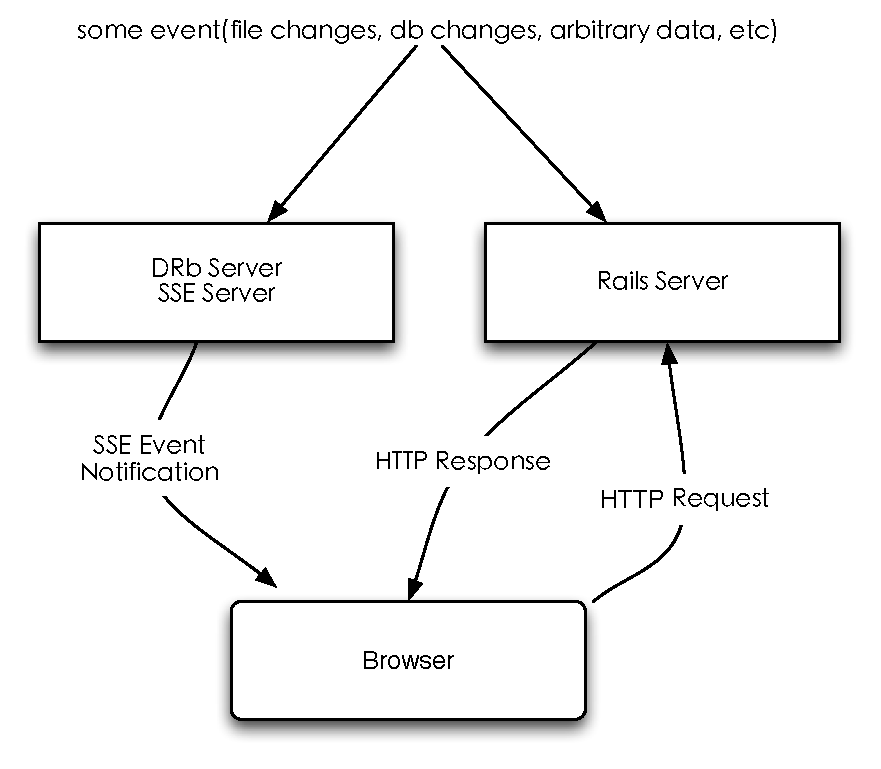
\includegraphics[width=0.7\textwidth]{images/overview/infrastructure.eps}
\caption{基础设施宏观示意图}
\label{fig-infra}
\end{figure}

在图\ref{fig-infra}中,可以看到,Rails消息总线技术主要涉及两方,共4大部件。在图\ref{fig-infra}的最上方是消息源,该部件负责产生消息,并借由Rails消息总线技术将 消息传递给浏览器客户端处。实际上,由于Rails消息总线技术是一门基础性技术,这里的消息源可能是由无数多种组件构成。按照目前实现计划,本文提供了两种消息源:其一是负责监控Rails工程目录下文件的变动,并将关键文件变动消息通知给浏览器客户端,这实际上是Auto-Reload技术的基础;其二则是负责对Rails服务器性能参数进行监控和收集统计,并将这些性能数据实时的传送至浏览器客户端,这实际上是Backend Instrumentation的技术基础。当然,数据源的种类不仅如此。实际上开发者还可以实现数据库的变动监控,一旦发觉数据库内的数据发生变动(比如通过Rails控制台改变),将立刻通知浏览器客户端进行刷新操作,从而即刻反映出后台数据库的变化对前端的影响。

第二大部件则是一个DRb Server组件。在一个典型的网页服务器后端,为了保证服务器的可用性及性能,开发者往往会使用服务器集群,用来均摊高昂的服务器压力,增强服务器的性能表现。同时,服务器后台一般是一个高并发的环境,可能有许多非服务器的进程作为工作子进程而工作。而这些工作子进程在处理用户请求之后,很有可能需要发送实时消息至用户的浏览器。考虑到操作系统进程间天然的隔离性,由于和用户的浏览器客户端通信的实体实际上是服务器进程,因此一般来说非服务器进程往往很难直接和浏览器之间进行通信。这个限制是和Rails消息总线的设计初衷箱违背的。为了解决这个问题,Rails消息总线技术引入了DRb Server部件。该部件负责后台中服务器进程和非服务器进程之间的通信,从而使得非服务器进程能够委托服务器进程向浏览器客户端发送相应的实时消息。

DRb Server不会直接和浏览器客户端通信,它会使用SSE Server模块向浏览器客户端发送消息。SSE Server的设计目标便是提供一套标准的、健壮的服务器到浏览器通信机制。它提供了两套模式,其一是Raw Streaming模式,用于直接向客户端发送原始数据,另一个是SSE Mode,用于和客户端使用HTML5 SSE标准协议进行通信,其稳定性和健壮性要优于前者。

最后,为了使得整个机制能够运转正常,还需要浏览器客户端方面的支持。实际上,第四大部件严格意义上来讲并不属于Rails消息总线技术。它实际上是位于浏览器客户端中的JavaScript脚本,用于接收SSE消息,并且指导浏览器针对不同的消息产生不同的响应行为。

\subsection{SSE Server总体方案设计}
SSE负责和浏览器直接通信,并且能够支持实时的向浏览器传送数据。但是,由于Rails使用了Rack技术(一种服务器通用接口技术),使得Rails很难绕过Rack的限制,直接和浏览器客户端进行通信。不难发觉,为了实现数据能够实时的发送至浏览器客户端,传统的基于Rack技术的网页服务器响应流程已经不适用了,需要一种新的机制来实现之。幸运的是,Rack在1.5之后提出了一套新的服务器接口标准,使得开发者能够直接从Rack手中接手对客户端原始套接字的占有,从而直接操作原始套接字,实现消息的实时发送。为了了解这个技术,需要简要介绍一下经典的Rack服务器响应流程。典型的Rails服务器栈如图\ref{fig-server-stack}所示。

\begin{figure}[h]
\centering
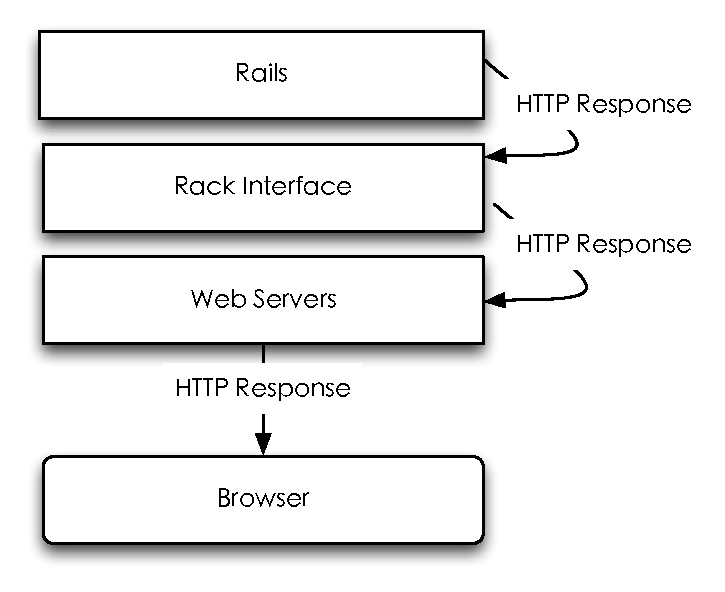
\includegraphics[width=0.7\textwidth]{images/overview/rack.eps}
\caption{典型的Rack服务器栈结构}
\label{fig-server-stack}
\end{figure}

在图\ref{fig-server-stack}中,可以看到,整个Rack技术是基于一种类似于堆栈的组织方式的。在这个服务器堆栈上,位于最顶端的是Rails服务器,其下则是Rack库代码,在之下则是各式各样的Web服务器。Rack技术的提出,主要便是为了解决开发者对代码精简的诉求和种类繁多的Web服务器接口之间的矛盾。Rack抽象出了一套基本的Web服务器接口,使其上层逻辑直接这套接口打交道。在下层,则是针对大量的不同服务器开发了为数众多的服务器适配接口。这样,使用Rack,开发者仅需要针对Rack的接口开发程序,便使得自己的程序能够兼容众多其他的服务器。

图\ref{fig-server-stack}展示了一套典型的Rack架构下的Web服务器工作示意图。可以看到,Rack技术的上层是任何需要适配网页服务器接口的组件,在这里我们以Rails为例。Rails是一个开源的网页服务器开发框架,因此需要支持不同种类的网页服务器。为了适配不同的网页服务器,Rails同过和Rack打交道,从而使用了一套标准的抽象服务器接口。当Rails希望向浏览器客户端发送HTTP响应时,它会首先通过Rack的抽象接口,将数据传递到Rack层,接着借由Rack内置的适配器,数据将被传送至底层实际的Web服务器处。最后,Web服务器将通过和浏览器客户端之间建立的原始套接字将数据(HTTP响应包)发送至浏览器。

通过以上的分析不难看出,典型的Rack架构提供了一套较为标准的数据传递路径,开发者很难对其进行定制。正是由于此,使得基于Rack的Rails技术很难凭借自身实现实时向浏览器客户端传递数据。而Rack劫持技术则是通过一种机制,使得上层的Rails能够直接通过Rack从Web服务器处将同客户端通信的原始套接字获取,尔后可以直接通过该套接字向浏览器传送数据,为实时消息推送创造了条件。

对比上述典型的Rack服务器堆栈结构,基于Rack劫持技术的服务器堆栈如图\ref{fig-rack-hijack}所示:

\begin{figure}[h]
\centering
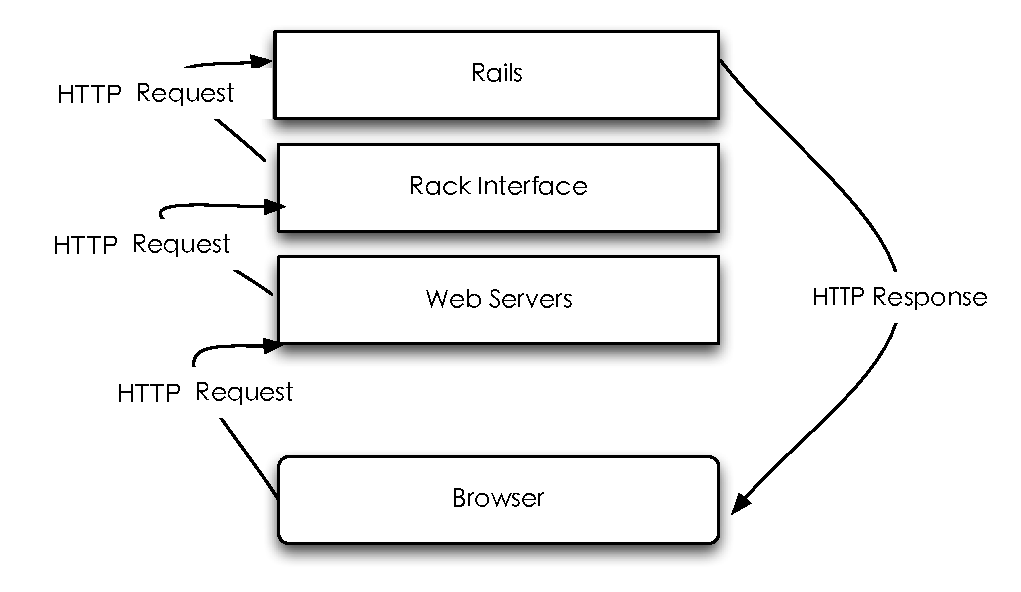
\includegraphics[width=0.7\textwidth]{images/overview/rack_hijack.eps}
\caption{Rack劫持技术原理示意图}
\label{fig-rack-hijack}
\end{figure}

可以看到,基于Rack劫持技术的服务器栈和一个传统的Rack服务器栈非常类似。Rack依旧承担解耦不同服务器接口差异的工作,HTTP请求的数据流动方式也依旧是沿Rack服务器堆栈向上传递。可以说,最大的不同就是HTTP响应数据的路径了。图\ref{fig-rack-hijack}清晰地展示了此时HTTP Response是如何传递的:Rails直接从Rack获取了同浏览器连接的原始套接字,于是Rails自己构造HTTP响应报文之后,直接将数据发送给了浏览器,而没有流经其下任何一层协议栈。不难看出,通过Rack劫持技术,Rails甚至可以实现非HTTP协议的数据报。在Rails消息总线技术中,本文依旧使用了HTTP协议,但是在Rails构建HTTP响应报文其间,本技术会实时将部分报文传递给浏览器客户端,从而实现数据的实时推送。

\subsection{DRb Server总体方案设计}

正如上一节所分析的,由于Rails运行的环境可能是由诸多集群服务器构成,并且即使统一台物理主机上亦可能存在多个工作进程。为了使得这些后台非服务器进程能够通过服务器进程和前端的浏览器进行通信,Rails消息总线技术提供了DRb Server技术用以实现将消息传递请求委托给相应的服务器进程技术。该技术的实现概况由图\ref{fig-drb}所示。

\begin{figure}[h]
\centering
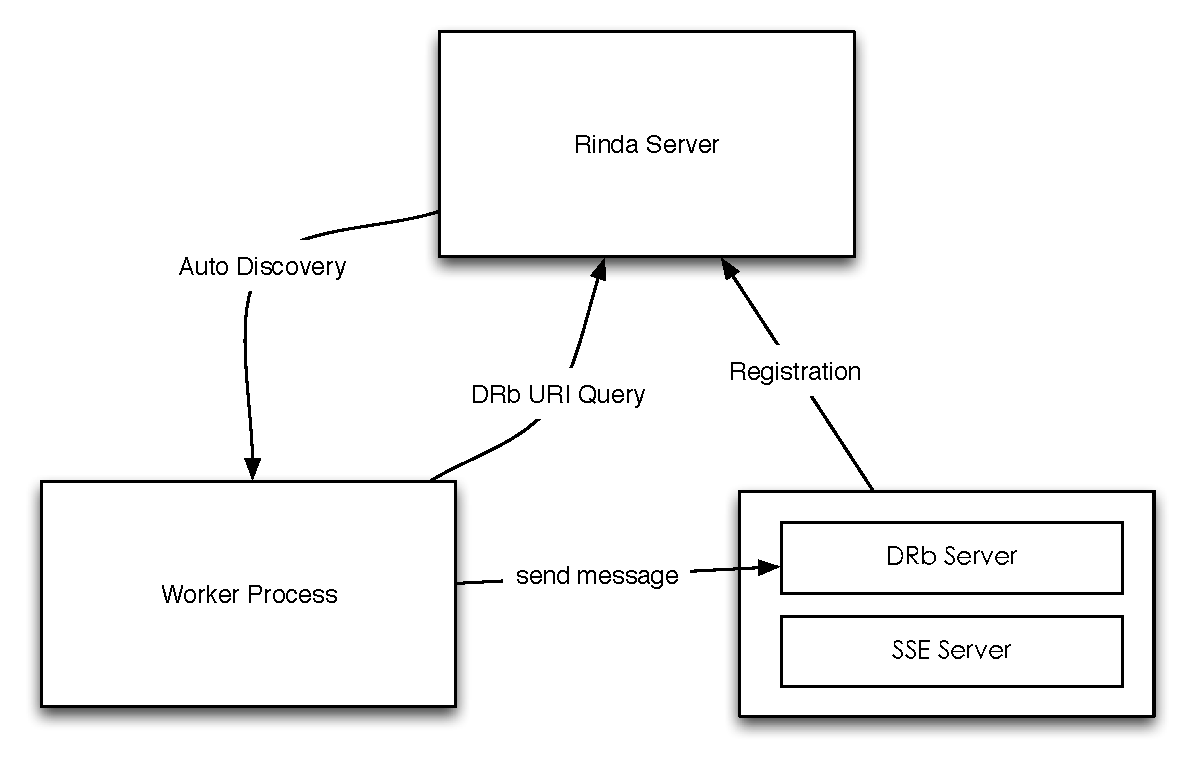
\includegraphics[width=0.7\textwidth]{images/overview/drb.eps}
\caption{Drb Server原理示意图}
\label{fig-drb}
\end{figure}

不难看出,DRb Server的设计实现主要由三大块组成。首先是DRb服务器模块,该模块负责接受来自于其他进程的请求,并且讲这个请求转发给后端的SSE Server,由该模块进行数据的发送。DRb服务器实际上是分布式Ruby(Distributed Ruby)的技术组成部分,通过DRb服务器,可以实现其他进程到该服务器所属进程的IPC(Inter-Process Call)调用。这样,位于后台工作进程的代码可以通过类似于本地调用一样的方式调用数据发送接口,而该接口会把参数和请求转发给DRb服务器,最终由位于服务器进程的DRb服务器将数据转发给浏览器客户端。

但是,如果仅仅使用DRb服务器会面临一个问题。该问题源于每一个DRb服务器实际上是基于原始套接字来实现进程间过程调用机制的,因此每一个DRb服务器都需要绑定一个网络地址。按照设计,Rails数据总线技术并没有使用一个特定的端口号和地址。这样做的目的是为了使得代码的部署更具有灵活性,但却带来了后台工作进程不知道如何寻找DRb服务器的问题。为了解决这个问题,Rails数据总线技术引入了Rinda技术。该技术同样是分布式Ruby解决方案中的一员,主要用于分布式系统中的主机发现。

Rinda服务器主要工作就是响应后台工作进程的连接请求,并向其提供本地注册在案的DRb服务器的网络地址和端口号。通过向Rinda服务器询问并获取这些信息,任意一个后台工作进程都能够随时连接到DRb服务器上并发送消息。这样做的好处是,使得DRb服务器不需要绑定到一个固定的地址和端口号,亦不需要服务器维护人员手动的配置地址参数,从而减少了人员工作量,同时增加了系统的灵活性。Rinda服务器起到了一个类似DNS服务器的作用,但是,其本身也需要被发现。基于同上的原因,Rinda服务器同样没有使用固定的网络地址和端口号,相反,Rinda服务器提供了一种自动发现(Auto Discovery)的机制,使得位于同一个局域网的工作进程能够发觉它的存在。该机制主要基于UDP的广播(Broadcast)机制,Rinda服务器通过监听并且接收来自于局域网内的广播消息来标识一个局域网内潜在客户。每一个后台工作进程会发送一个广播至局域网内,通过该种手段,便能够找到局域网内的Rinda服务器(如果该服务器存在的话)。当工作进程找到一个Rinda服务器后,便与其建立一个正式网络连接,并通过此链接获取该网内其他DRb服务器的基本信息。当然,同样的过程必须同时发生在DRb服务器身上。在一个DRb服务器启动并初始化完成后,它也会找到当前网内的Rinda服务器,并且向其注册自己的基本信息。值得注意的是,在同样一个局域网内,能通过Rinda服务器查询到的DRb服务器必须也是曾今向Rinda服务器注册过自己身份的DRb服务器。

最后,对于后台工作进程,当其通过Rinda服务器获取了目标DRb服务器的地址和端口号之后,便能够通过分布式Ruby技术使用IPC通信机制向服务器发送请求,委托服务器向客户端发送实时消息。


\subsection{Auto Reload总体方案设计}

Auto Reload技术旨在监控服务器后端的变动,并且在开发模式下通知前端浏览器做出相应的刷新动作。其具体实现细节详见图\ref{fig-reload}:

\begin{figure}[h]
\centering
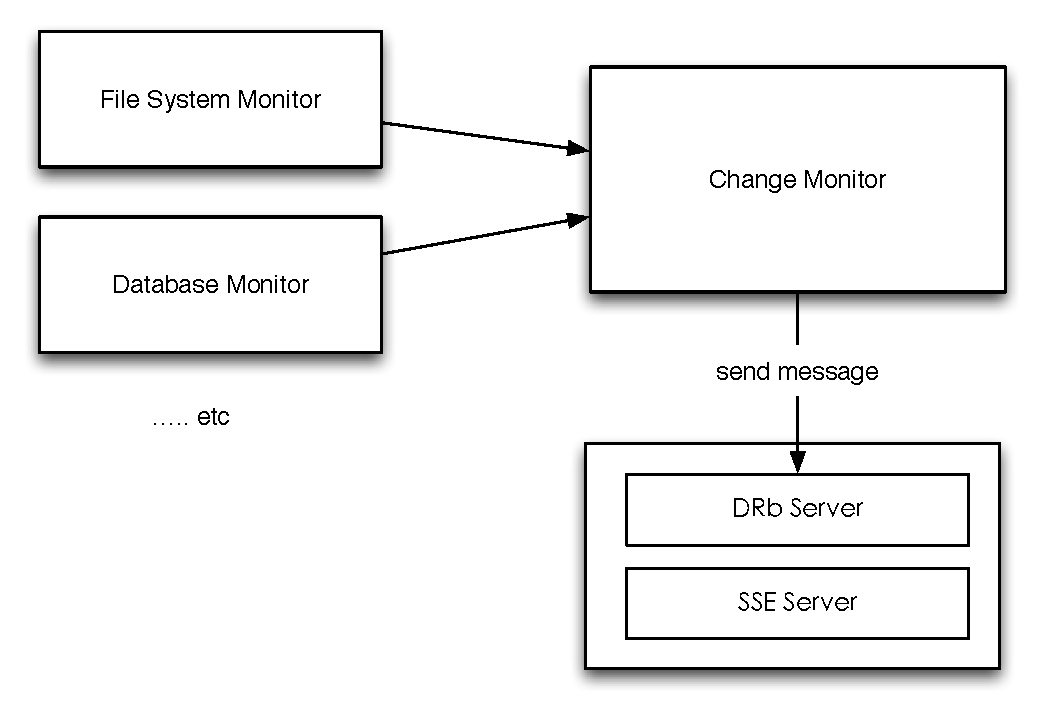
\includegraphics[width=0.7\textwidth]{images/overview/auto_reload.eps}
\caption{Auto Reload原理示意图}
\label{fig-reload}
\end{figure}

不难看出,Auto Reload是紧密依赖于Rails消息总线技术中的DRb Server技术和SSE Server技术的。Auto Reload拥有一个统一前端,该前端负责和相应的DRb服务器打交道。目前,Auto Reload包括两个变动消息源,一个负责监控文件目录变动,另一个则负责监控Rails后台数据库变动。当其任意一方捕获到变动后,将会向其对应的前端Change Monitor发送消息。当前端Change Monitor接收到来自于各个数据源的消息之后,便会通过DRb Server以远程过程调用的方式请求DRb服务器向客户端发送消息,并且通过进程间通信机制将消息体数据传送给DRb服务器所在的网页服务器进程之中。

对于文件系统监控模块,本系统使用了基于本地码的Ruby拓展。该拓展能够监控指定目录及其子目录下所有文件系统节点的变动,一旦发生任何变动便会通知该模块。该模块将首先对信息进行筛选,让合法的并且被关注的文件变动消息得以传递,并且该模块会将消息体本身封装为Auto Reload子模块内部通用的消息结构。从而让各个数据源和消息类型能够以统一的方式在子系统内传递。

另一个则是数据库监控模块。该模块主要用于监控Rails服务器后台数据库的变动,一旦任何数据发生改动,它都会通过统一前端通知DRb服务器告知浏览器这一变动。从而使得浏览器更为灵活快捷的响应后台变化。值得注意的是,数据库变动监测逻辑并不是实现于数据库层面的。虽然是现在该层面有着运行效率较高的优点,但是该方法需要对大量数据库种类进行适配的要求足以抵消其优势。鉴于Rails开发框架下,开发者主要通过ActiveRecord(Rails提供的统一数据库接口)技术同数据库打交道,故而考虑到通用型,Auto Reload将数据库监控逻辑实现到了该层面。通过监控ActiveRecord模块的活动,从而获知开发者或者代码对数据库的变动。

\subsection{Backend Instrumentation总体方案设计}
Backend Instrumentation技术负责收集Rails后台运行性能参数,加以统计和简单处理,并通过实时方式将其传送到前端浏览器。该技术是Rails基于网页的控制终端的支撑技术之一。Rails网页控制终端是供服务器维护者远程管理和配置Rails后台服务器的一种技术,相比起基于桌面客户端的终端,网页控制终端具有无需安装、部署和升级简单、快捷等优势。而Backend Instrumentation技术则是该终端负责实时获取性能参数的支撑技术,对Rails来说具有较高的必要性。该技术的基本架构如下图所示:

\begin{figure}[h]
\centering
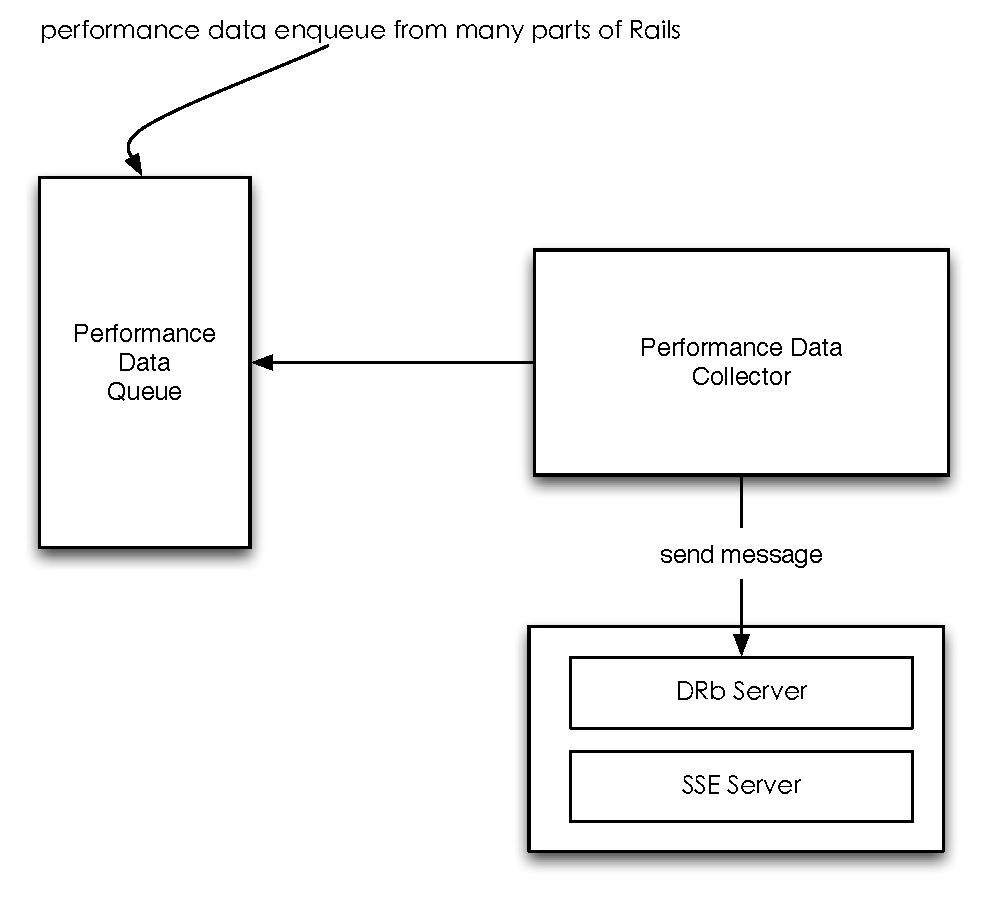
\includegraphics[width=0.7\textwidth]{images/overview/backend_instrumentation.eps}
\caption{Backend Instrumentation原理示意图}
\label{fig-back-instrumentaion}
\end{figure}

该技术结构和Auto Reload特性类似,依旧依赖于Rails消息总线技术中的DRb Server技术和SSE Server技术。在一个刷新周期内,Performance Data Collector会将收集到的性能数据通过消息总线传送至前台浏览器。浏览器接受到相应的性能数据,能够以较为直观的方式将其展示出来。Performance Data Collector的数据来源于Performance Data Queue,前者周期性地从后者处获取实时性能数据。之所以需要这个消息队列,是由于目前Rails收集性能参数的关键点较多,本系统使用这个队列,使得散落Rails各地的性能测试点产生的数据能够被集中起来,以便于统一管理和获取。

\section{系统逻辑结构设计}
为了在上一节基础上进一步阐述Rails消息总线技术各部分的实现机理,本文将在本小节中详细描述各大部件的逻辑结构和运行机制,以期能够展示出整体系统的工作流。本节首先将通过包图的形式介绍Rails消息总线技术总体上的逻辑结构,并通过时序图的方式介绍各大部件之间的交互流程。然后将对主要部件的逻辑结构和工作流程进行详细介绍。通过上述两方面的介绍,详尽描述Rails消息总线技术的逻辑层面的结构设计。
\subsection{总体结构和工作流}
Rails消息总线技术从逻辑上来划分,共分为下述六大模块,每个模块用一个包表示,如图\ref{fig-overall}:

\begin{figure}[h]
\centering
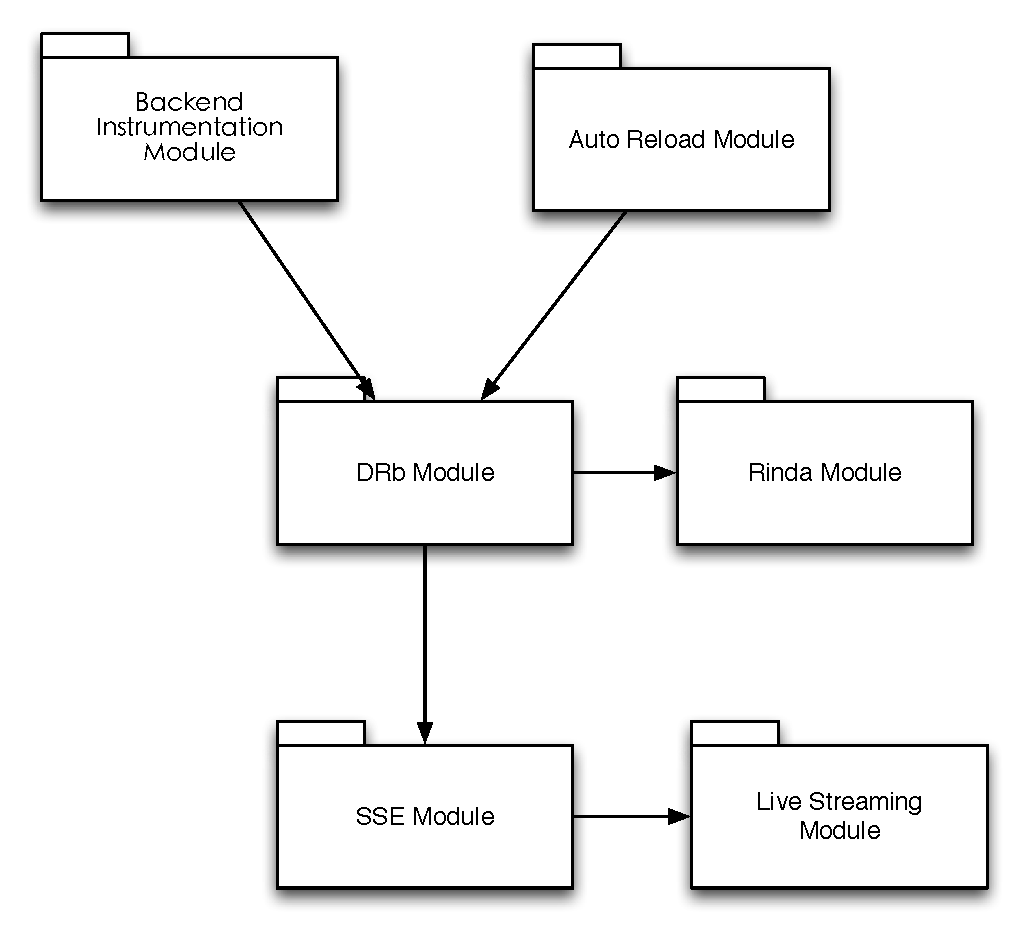
\includegraphics[width=0.7\textwidth]{images/overview/overall_logic.eps}
\caption{Rails消息总线技术总体包图}
\label{fig-overall}
\end{figure}

图\ref{fig-overall}展示了本项目宏观上的逻辑结构图。可以看到,Rails 消息总线技术的核心在于图\ref{fig-overall}的第二层和第三层,由这两个层次共同提供了一套面向Rails框架内部的服务器实时消息推送机制,以实现从服务器到浏览器的单向实时通信。而对于图\ref{fig-overall}的最上面一个层次,则是作为核心技术的实现示例,和Rails其他部分的依赖的技术而存在的。这一层分别实现了Auto-Reload技术和Backend Instrumentation技术,并且依赖于下面的核心层将相应数据发送至了浏览器客户端。

由上而下这些模块分别的工作是:Backend Instrumentation模块,获取服务器后台实时性能数据,并将该数据实时传递至前端浏览器;Auto Reload模块,监控Rails工程目录文件变动,并通知浏览器刷新页面;DRb模块,负责服务器后端进程间通信,通过远程过程调用响应后台进程的请求;Rinda模块,负责接收DRb服务器的注册信息,并向客户提供DRb服务器的地址及端口号,同时提供服务器自动发现机制;SSE模块,负责实现HTML5 中的SSE协议,向浏览器客户端发送SSE消息;Live Streaming模块,负责劫持Rack原始套接字,提供向浏览器输出实时数据的可能性。

为了清楚的描述这些部件的动态行为,以及它们之间是如何交互的,图\ref{fig-overall-timing}将以时序图的方式展示之:

\begin{figure}[h]
\centering
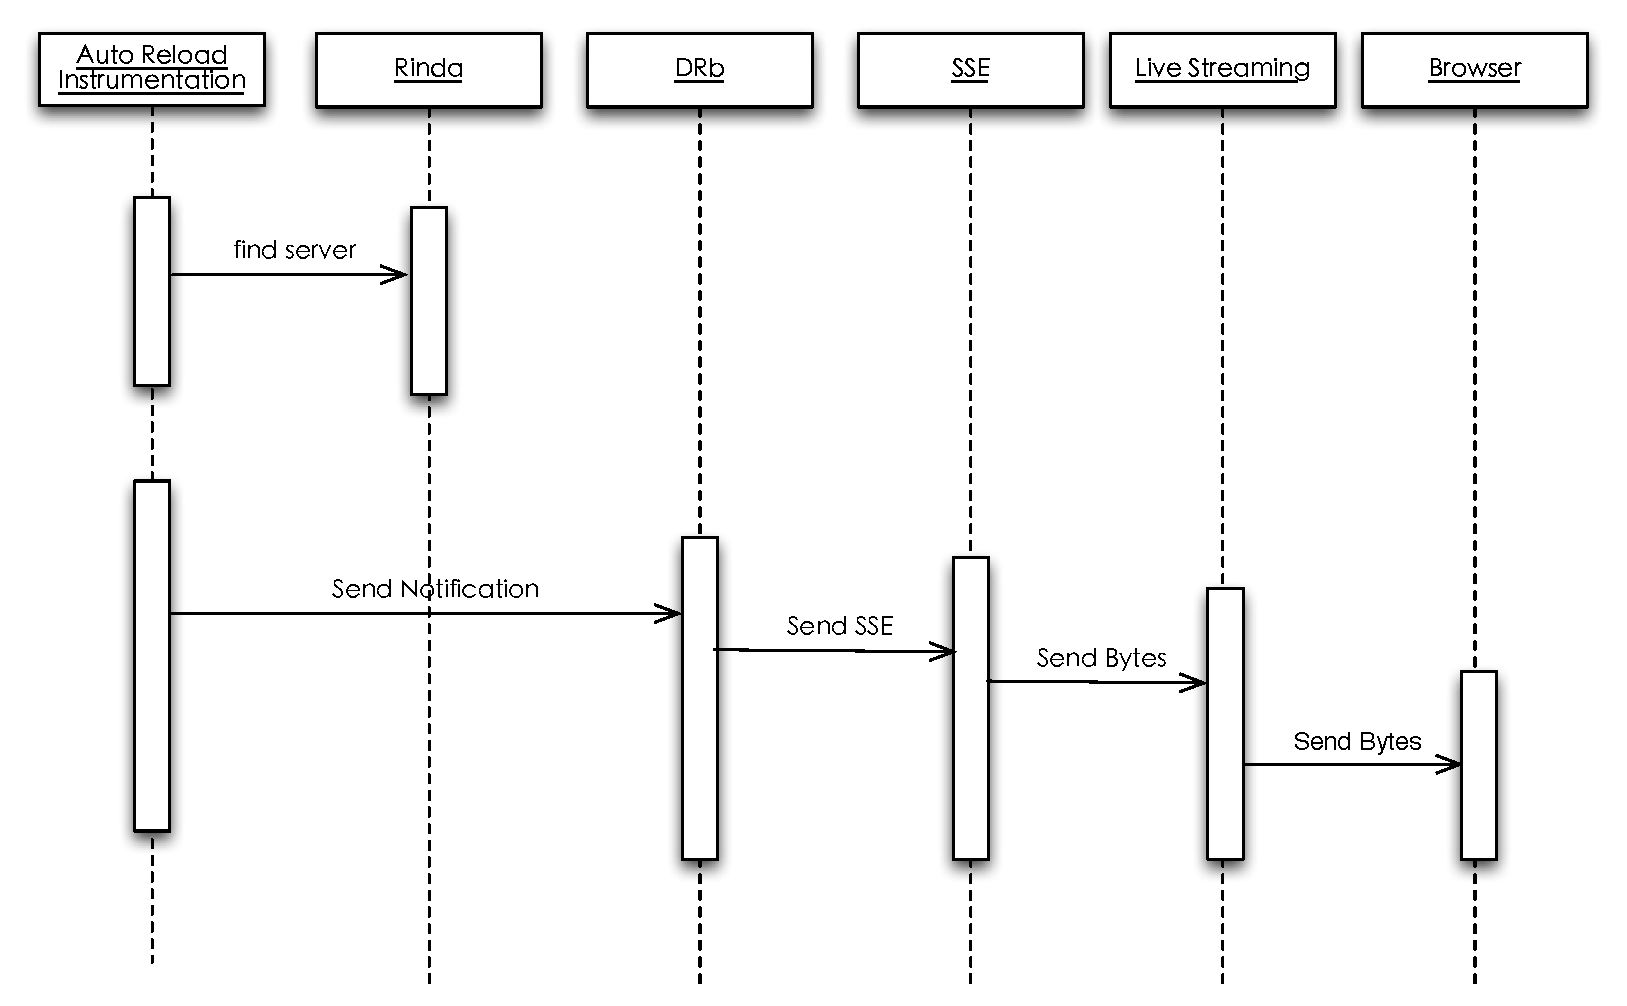
\includegraphics[width=\textwidth]{images/overview/overall_timing.eps}
\caption{Rails消息总线技术各模块交互时序图}
\label{fig-overall-timing}
\end{figure}

可以看到,整个序列当中,任何事件的发起者都是Auto Reload模块和Backend Instrumentation模块了。在这两个模块初始化的的时候,他们都会向本地局域网中发送消息,以寻找本地局域网中的Rinda服务器,当其找到Rinda服务器之后,便会向其查询本地网络中的RDb服务器(这里省去了DRb服务器向Rinda注册自身的过程),这时候便能够通过Rinda返回的网络地址向DRb服务器发送请求了。

接下来,若Auto Reload触发一个文件系统节点变动的消息,或是Backend Instrumentation达到一个新的采样时间点时,它们将会组织信息,并将统一格式的消息发送给DRb服务器。这时候,DRb服务器接受到来自于其他进程的远程过程调用请求,作为响应,它将会把作为参数的具体消息内容传送给SSE模块,通过其传送给浏览器客户端。

当SSE接受到请求之后,它将把统一的消息格式拆封,同时将消息体中的具体信息和数据提取出来,并组件新的SSE消息结构。根据当前和浏览器客户端的连接情况,SSE模块会设置SSE消息体的控制参数(例如消息序列号、重连机制等)。当SSE消息体构建成功之后,SSE模块将通知Live Streaming模块准备数据的传送,后者在接收到SSE消息体之后,将其序列化成字节流,并通过同浏览器客户端之间的原始套接字将数据发送至浏览器处。当然,这里依旧省略了Live Streaming模块劫持Rack原始套接字的过程。

以上过程,便是Rails消息总线技术的一个典型的流程,通过对这个过程的描述,反应了本项目各个模块之间具体的职责和交互方式,下面将就每个具体模块进行介绍。

\subsection{DRb和Rinda模块的逻辑结构}
DRb和Rinda模块主要负责将非服务器进程的数据传输请求委托给服务器进程,其主要包括如下几个模块:

\begin{figure}[h]
\centering
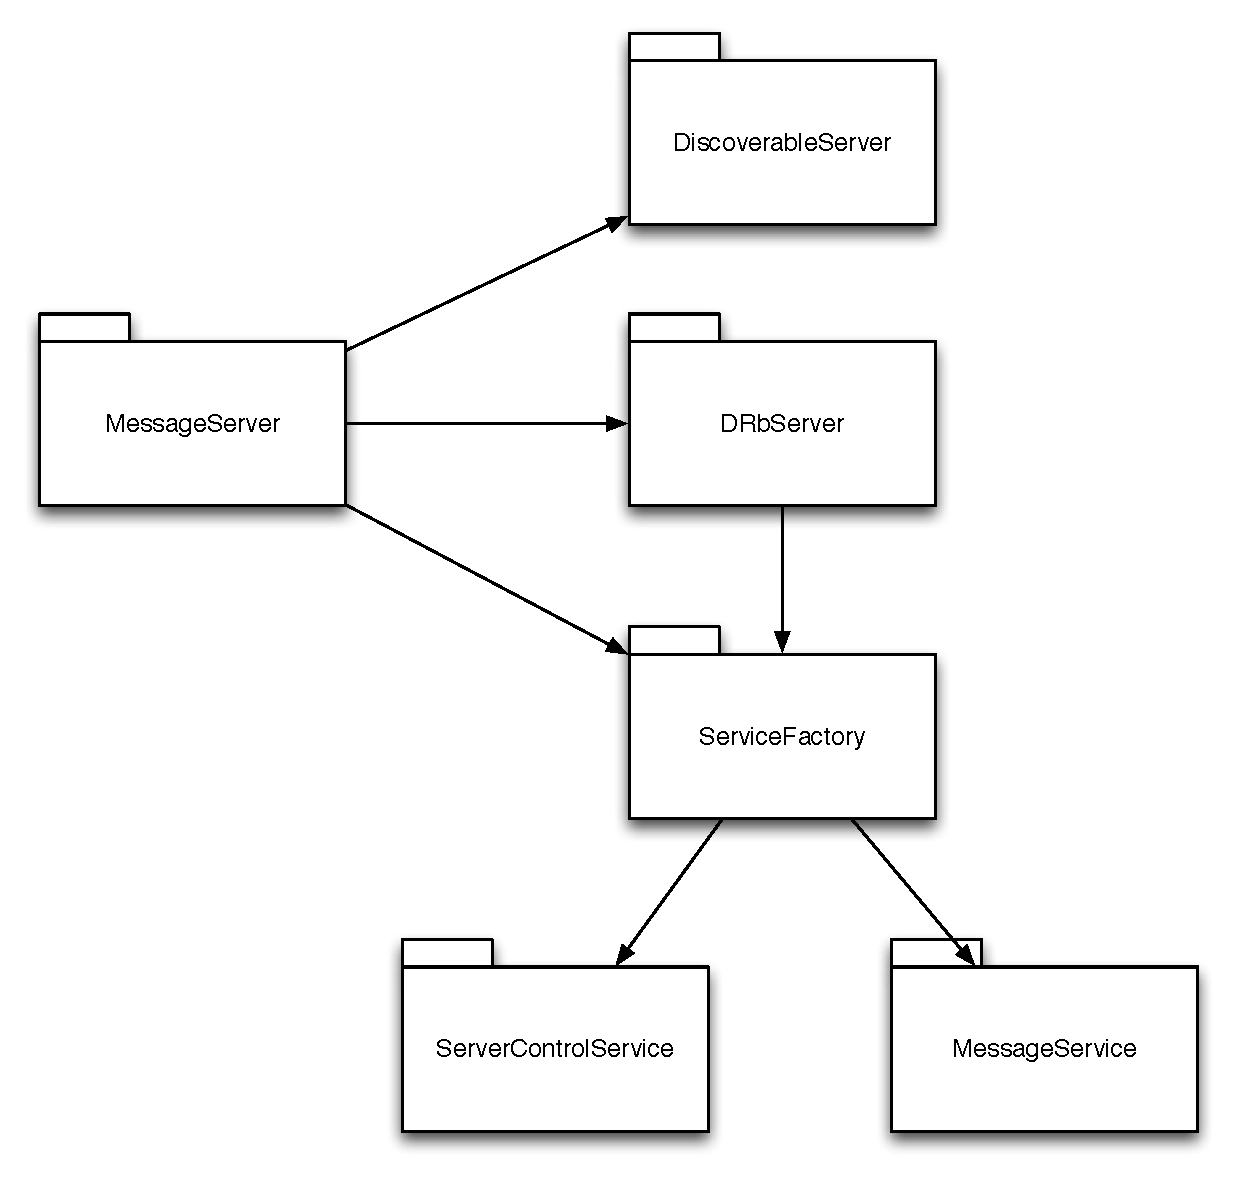
\includegraphics[width=0.7\textwidth]{images/overview/drb_rinda.eps}
\caption{DRb及Rinda模块逻辑结构图}
\label{fig-drb-rinda}
\end{figure}

图\ref{fig-drb-rinda}主要包含七大模块,其分别的作用如下:MessageServer作为DRb技术的客户端,客户进程通过该模块连接DRb服务器,并且发起以此远程过程调用;DiscoverableServer实际上是一个Rinda服务器,通过它可以注册DRb服务器的信息,并且告知客户端其查询的DRb服务器的地址。DRbServer则是具体的响应远程过程调用的服务器,它部署在服务器进程中,并且帮助客户在其所在进程中执行远程代码;ServiceFactory是作为DRb技术的FrontObject的对象,它实际上是一个工厂,客户端通过它获取该服务器提供的各种远程服务;ServerControlService是ServiceFactory工厂提供的远程服务之一,它的主要目的是给客户端提供一个接口,使得其能够远程控制当前DRb(暂停、关闭等);MessageService是ServiceFactory工厂提供的另一个远程服务,它的提供了发送消息的服务,客户端可以通过该服务向浏览器发送实时消息。

图\ref{fig-drb-rinda-timing}展示了这些类是如何交互的:

\begin{figure}[h]
\centering
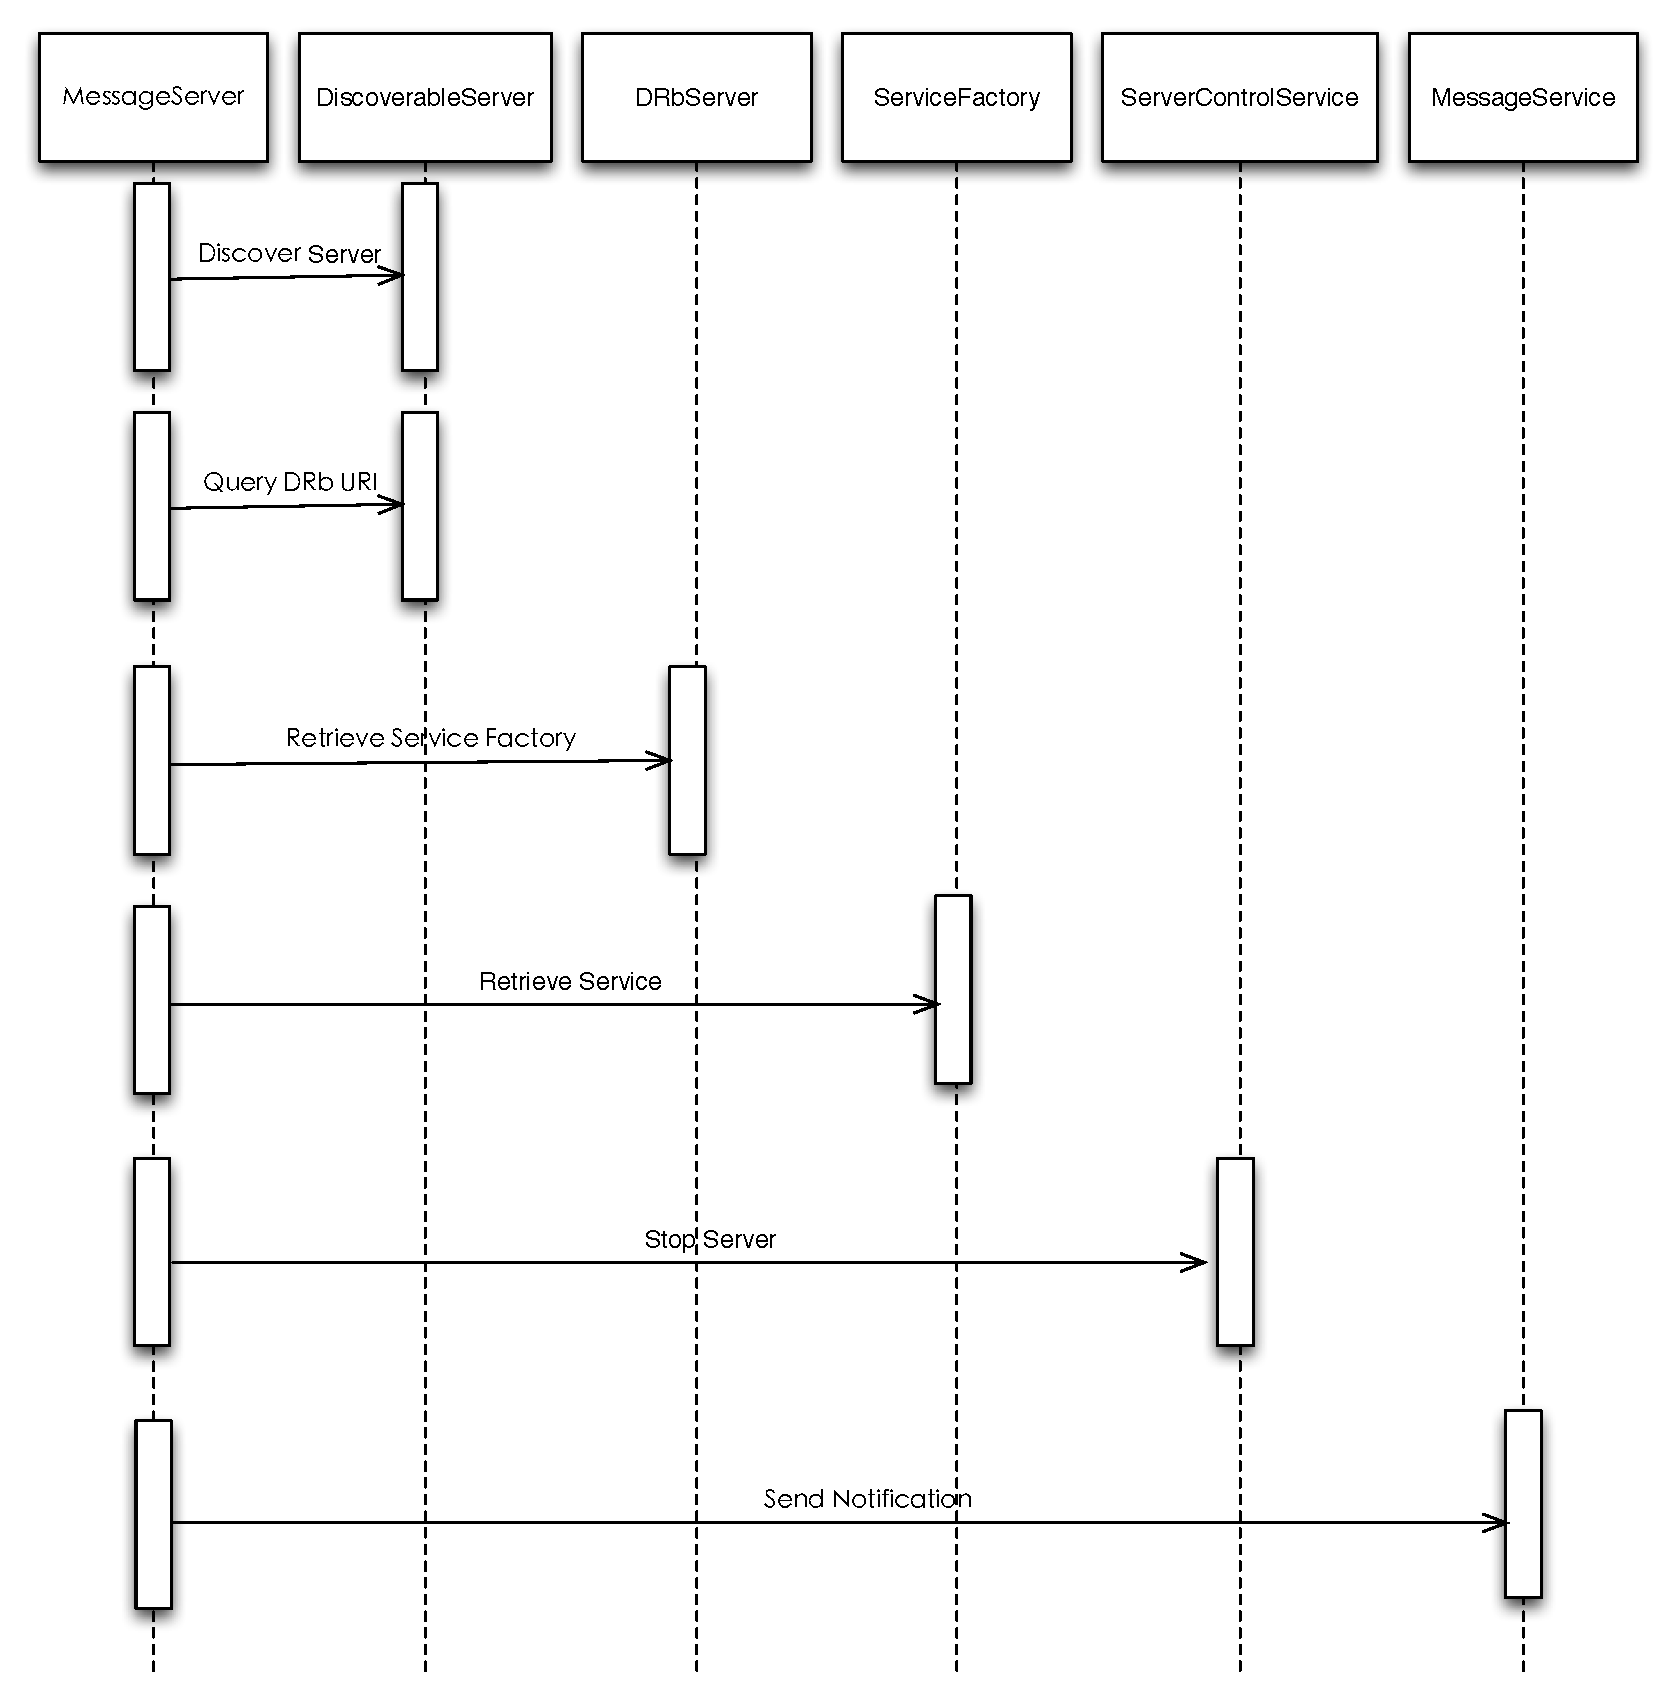
\includegraphics[width=\textwidth]{images/overview/drb_rinda_timing.eps}
\caption{DRb及Rinda模块交互时序图}
\label{fig-drb-rinda-timing}
\end{figure}

可以看到,在整个机制流程中,MessageServer是负责驻留在客户端进程,发现DRb服务器,并且向其发送消息。它是客户端向DRB服务器通信的总接口。在初始化的时期,MessageServer将会向本地局域网发送一条广播消息,以寻找本地局域网络中的Rinda服务器。在本系统中,Rinda服务器是由DiscoverableServer模块来实现的,当DiscoverableServer接收到该条消息之后,便会告知MessageServer自己的存在。MessageServer发现DiscoverableServer之后,便开始向其查询本地存在的DRb服务器,这时候DiscoverableServer便会将之前注册在案的DRb服务器地址告知于MessageServer。

MessageServer在获取了DRb服务器的地址后,便会尝试连接该服务器。如果成功,MessageServer将会尝试从DRb服务器处获取一个前端对象(Front Object)。在本系统中,DRb服务器是由DRbServer模块实现的,作为响应,DRbServer将会向MessageServer返回一个ServiceFactory对象。ServiceFactory是作为一个服务的统一接口存在的,它会给客户端返回其请求的服务接口。MessageServer可以请求一个ServerControlService服务对象,通过其控制该台DRb服务器的运行状态,亦可以请求一个MessageService服务对象,通过其向DRb服务器发送实时消息。

在MessageServer获得任何一个服务对象之后,便可以通过该对象向服务发送请求了。ServerControlService服务可以接受一个控制命令,用以停止当前DRb服务器的运行,而MessageService提供了一个发送消息的接口,客户端可以通过该接口发送一条消息,该消息将被MessageService打包发送给SSE模块,从而最终实时地发送给浏览器客户端。

\subsection{SSE模块的逻辑结构}
SSE模块主要负责实现HTML5的SSE标准协议,为Rails上层部件提供标准SSE接口支持。该模块的结构如图\ref{fig-sse-module}所示:

\begin{figure}[h]
\centering
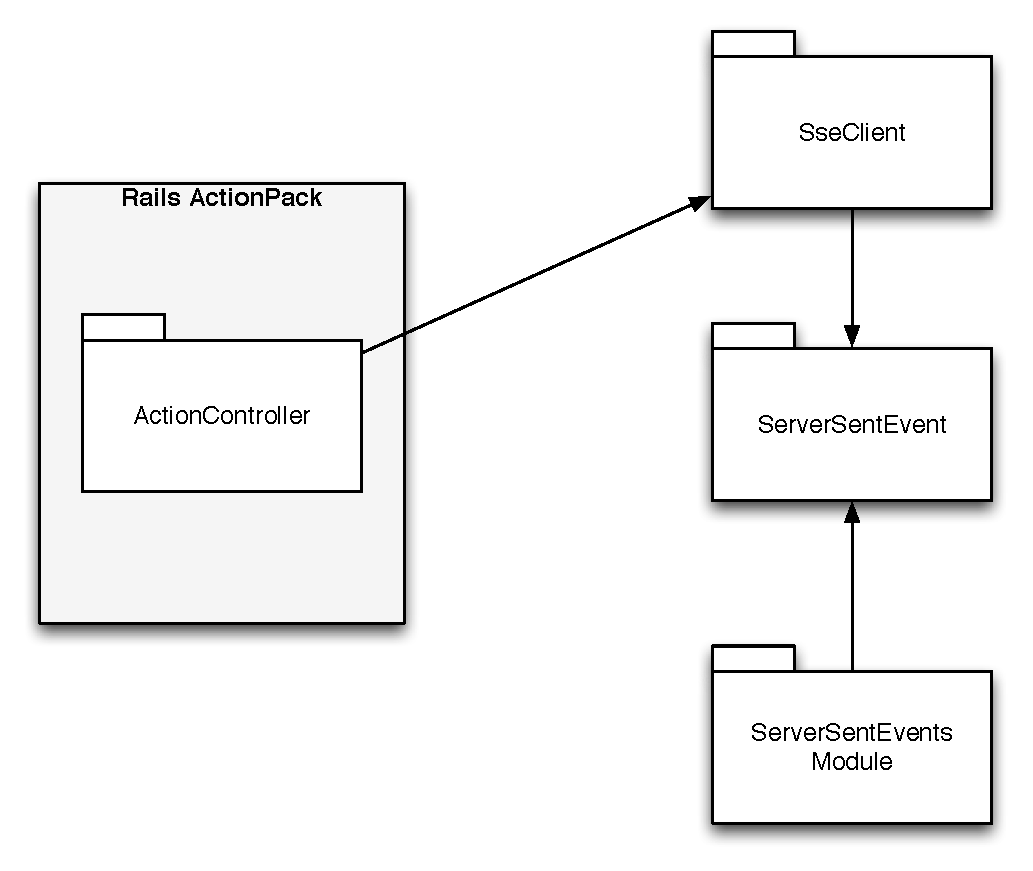
\includegraphics[width=0.6\textwidth]{images/overview/sse_module.eps}
\caption{SSE模块逻辑结构图}
\label{fig-sse-module}
\end{figure}

在图\ref{fig-sse-module}中,最右边的模块属于Rails现有的模块,而本技术的SSE模块则是直接作用于Rails的ActionController模块。Rails的设计理念中大量推崇了所谓MVC设计模式,通过控制器来从模型处获取实际数据,并将得到的数据传送给视图,再从视图处得到界面展示信息,最终向用户显示出界面。而ActionController模块则是Rails实现的MVC框架中其控制器作用的部件。传统上,每当一个新的页面请求发至相应的控制器时,ActionController会和ActionView和ActiveRecord打交道,并生成数据和展示视图返回给客户端。但是,在应用了Rails消息总线技术后,ActionController将直接把请求转发给SSE模块,并委托SSE模块处理客户端请求。这样,通过从ActionController夺取对浏览器客户端自由发送数据的权限,SSE模块实现了实时的消息发送。

图\ref{fig-sse-module}的右边则是组成SSE模块的三大子模块。它们分别的作用是:ServerSentEvents Module,负责提供统一接口,并且提供API共开发者调用;ServerSentEvent是封装SSE消息的一个对象,开发者需要在其初始化时提供欲传递的数据,并将其交给公共接口以发送至客户端,ServerSentEvent同时也是本模块内部对SSE数据结构的表示方式;SseClient则是整个模块中真正负责实现SSE逻辑的模块,该模块负责接收待发送的ServerSentEvent消息结构,生成标准SSE数据流表示方法,生成消息ID等诸多任务。

为了更加清晰地展示这些模块之间的动态行为,图\ref{fig-sse-module-timing1}提供了其运行时的时序图:

\begin{figure}[h]
\centering
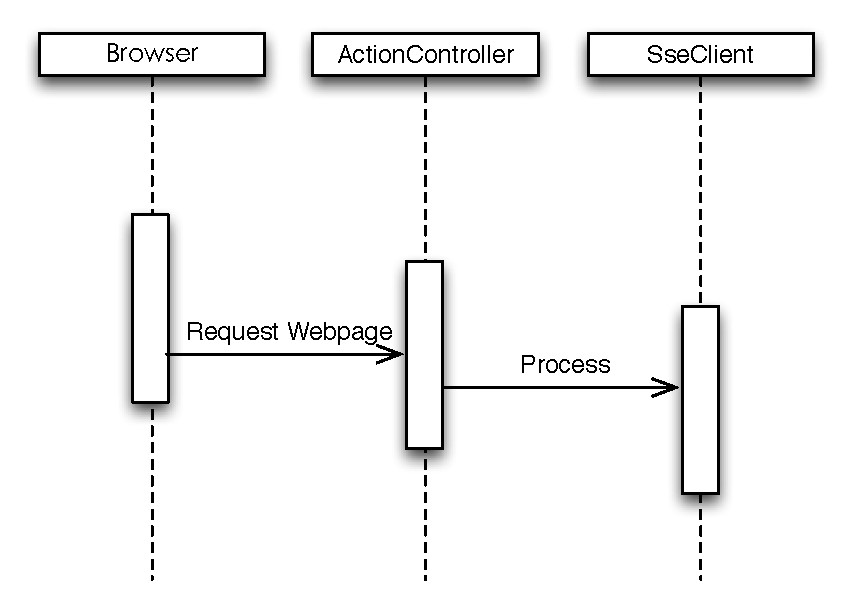
\includegraphics[width=0.7\textwidth]{images/overview/sse_module_timing1.eps}
\caption{浏览器连接过程时序图}
\label{fig-sse-module-timing1}
\end{figure}

可以看到,首先浏览器向服务器请求一个网页数据,经由Rails的路由机制,该请求被转发给了相应的控制器。此时,控制器不会像传统Rails程序一样调用视图和模型的相应代码,而是将该请求的处理委托给SseClient处理,SseClient接收到请求后,会开始长等待,直到其他模块告知需要传送消息给客户端时方才激活。此时,控制器和浏览器客户端再无关系,而是直接由SseClient以服务器的名义和客户端通信。另外,为了了解发送消息时的过程,图\ref{fig-sse-module-timing2}展示了发送消息的时序逻辑:

\begin{figure}[h]
\centering
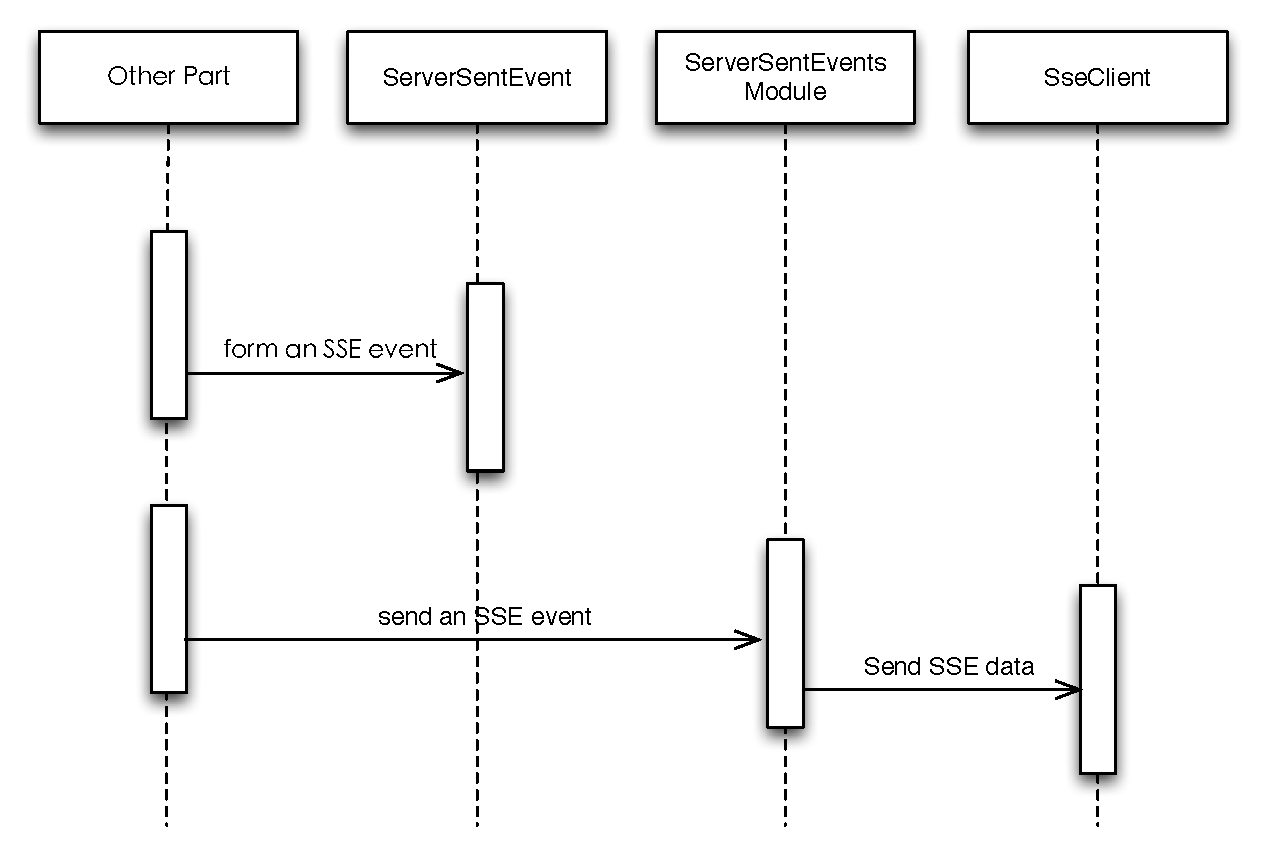
\includegraphics[width=0.8\textwidth]{images/overview/sse_module_timing2.eps}
\caption{SSE消息发送过程时序图}
\label{fig-sse-module-timing2}
\end{figure}

在图\ref{fig-sse-module-timing2}中,任何一个SSE消息的发起过程都源于本系统之外的某个组件的请求。当某个组件需要向客户端发送消息时,它首先将构建一个ServerSentEvent数据结构,并将消息数据封装于其中。这之后,通过向ServerSentEvents Module传送这个ServerSentEvent对象,使得ServerSentEvents Module发送该条SSE消息。ServerSentEvents Module拿到一个ServerSentEvents之后,会将其直接传送给SseClient。SseClient会对该条消息进行处理(添加序列ID、重连命令等),然后序列化成字节流,最后将该串字节流发送至浏览器客户端处,从而实现了实时SSE消息的发送。


\subsection{Live Streaming模块的逻辑结构}
Live Streaming模块主要负责利用Rack劫持技术获取客户端原始套接字,从而实现向客户端的实时数据传输。该模块的主要结构如图\ref{fig-live}所示:

\begin{figure}[h]
\centering
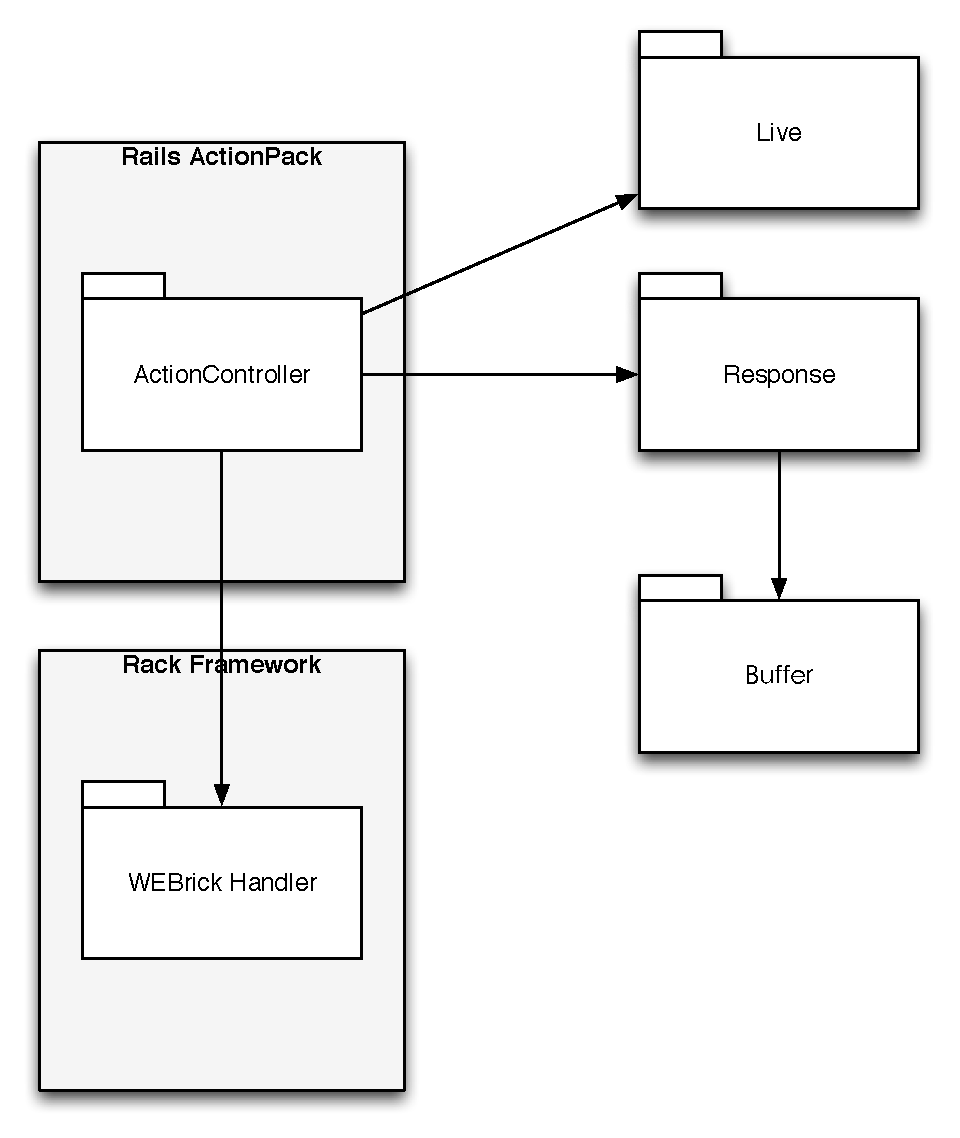
\includegraphics[width=0.7\textwidth]{images/overview/live_streaming.eps}
\caption{Live Streaming模块逻辑结构图}
\label{fig-live}
\end{figure}

图\ref{fig-live}展示了Live Streaming模块的各大部件。其中ActionController是Rails实现MVC模式中控制器的模块,该模块属于Rails既有模块。可以看到,Live Streaming模块主要是有四大部件构成的,它们分别的功能如下:Live模块负责覆盖ActionController原有行为,特别是其用于处理客户端请求的process方法,Live提供了一套基于Rack劫持技术的解决方案,以使得数据能够绕过Rails和Rack被实时的传送到浏览器客户端;Response对象用于封装一个HTTP响应,但由于此时HTTP响应已经不再是预先构造好再传送,该对象替换了Rails原有Response实现,提供了实时的构建和即时传输数据功能;Buffer用于提供一个缓冲区,该缓冲区用于提高IO效率,并且更是为了适配Rails原有接口;WEBrick Handler用于实现WEBRick服务器的Rack劫持技术,由于Rack劫持技术属于一套标准,目前支持该标准的浏览器数量尚有限,因此为了本项目能够顺利实施,这里针对Ruby内置的服务器WEBrick自行实现了Rack劫持标准,使得本项目能够在实践中被应用。

Live模块通过以下方法实现了数据的实时传递:当浏览器客户端向Rails服务器获取数据时,控制器的process负责处理并且响应这一请求,Live模块覆盖了控制器的process方法,因此获取了响应客户端的主动权。这之后,Live使用本模块实现版本的Response对象并将其作为参数传递给下层的Rack,同时根据Rack劫持协议告知Rack使用该对象进行响应。Rack使用WEBRick Handler响应客户端,由于此时Response是本模块实现的,因此这里使得Rack所在线程被阻塞,直到上层向Response写入数据或者由于数据流被关闭产生了异常。可以看到,控制和客户端通信的原始套接字所在的线程总是会阻塞,但当有数据写入时,该线程又会运行并将新的数据发送给客户端,由此实现了数据的实时传递。


\subsection{Auto Reload模块的逻辑结构}
Auto Reload负责检测Rails工程目录下的文件变动,并通知浏览器该项变动。其主要结构如图\ref{fig-reload-struct}所示:

\begin{figure}[h]
\centering
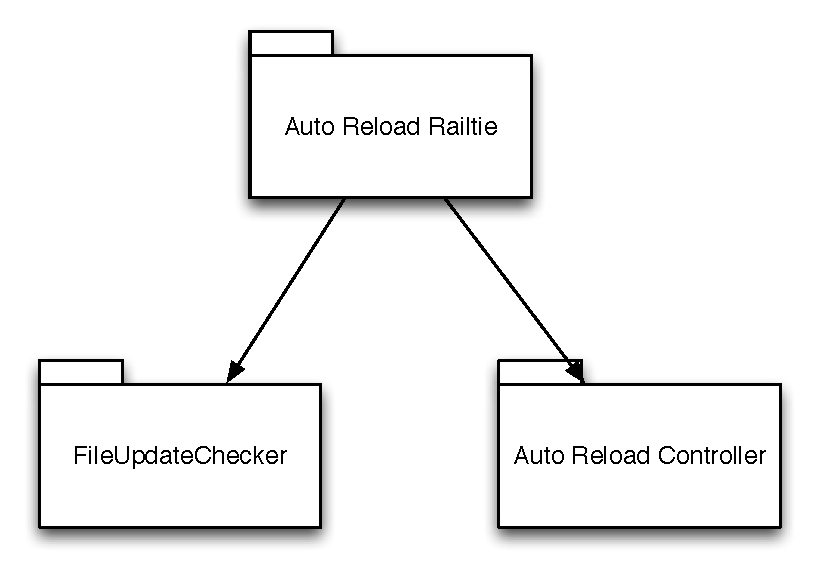
\includegraphics[width=0.7\textwidth]{images/overview/auto_reload_struct.eps}
\caption{Auto Reload模块逻辑结构图}
\label{fig-reload-struct}
\end{figure}

不难看到,Auto Reload模块主要是由三个部分构成的,这三个部分的作用分别如是:Auto Reload Railtie是一个Railtie实例,它作为一个Railtie,使得整个Auto Reload模块能够作为Rails的插件形式被载入和初始化。在初始化时,该模块负责判断当前环境,如果发觉是服务器环境,则载入相应代码逻辑并初始化其状态,若发觉是控制台环境,则避免载入代码逻辑;FileUpdateChecker则是负责监视Rails工程目录文件系统变动的模块,该模块会不断获取监控目录下的文件集合,并且与历史集合进行比对,从而发觉前后文件节点的变动,该方法具有很高的可移植性,适用于OS X、Linux以及Windows等平台;Auto Reload Controller则是负责发送文件变动消息的接口,它是负责Rails服务器和浏览器客户端通信的总接口,浏览器通过该模块接收SSE消息,服务器通过该模块发送相应文件变动消息。

在Rails工程初始化时,Auto Reload Railtie首先将自己注册到Gemfile里,则会在其后被Rails自动载入,并调用其初始化接口进行初始化工作。Auto Reload Railtie初始化的第一步是判断自己是否运行在Rails服务器中,只有运行在服务器模式下,Auto Reload Railtie方才会载入Auto Reload模块的其他组件,并进行相应的初始化工作。当Auto Reload Railtie完成初始化后,整个Auto Reload系统便宣告正常工作。这时候FileUpdateChecker将开始监视Rails工程目录,通过比对前后文件树的变化,FileUpdateChecker能够查知文件系统的任何变化。一旦FileUpdateChecker发现了文件系统有所变动,它便会通过DRb告知服务器这一变动,DRb则会通知SSE模块将这一消息传递给浏览器客户端。这之后,Auto Reload Controller作为与浏览器客户端通信的代表,将会将这一消息序列化为字节流,并且实时地传递给前端浏览器。至此,浏览器便接收到来自于后端的文件系统变动消息,并作出相应响应(一般来说是刷新整个页面)。

\subsection{Backend Instrumentation模块的逻辑结构}
Backend Instrumentation负责实时地收集Rails服务器性能数据,并将该数据实时地传送给浏览器。其主要结构如图\ref{fig-instrument-struct}所示:

\begin{figure}[h]
\centering
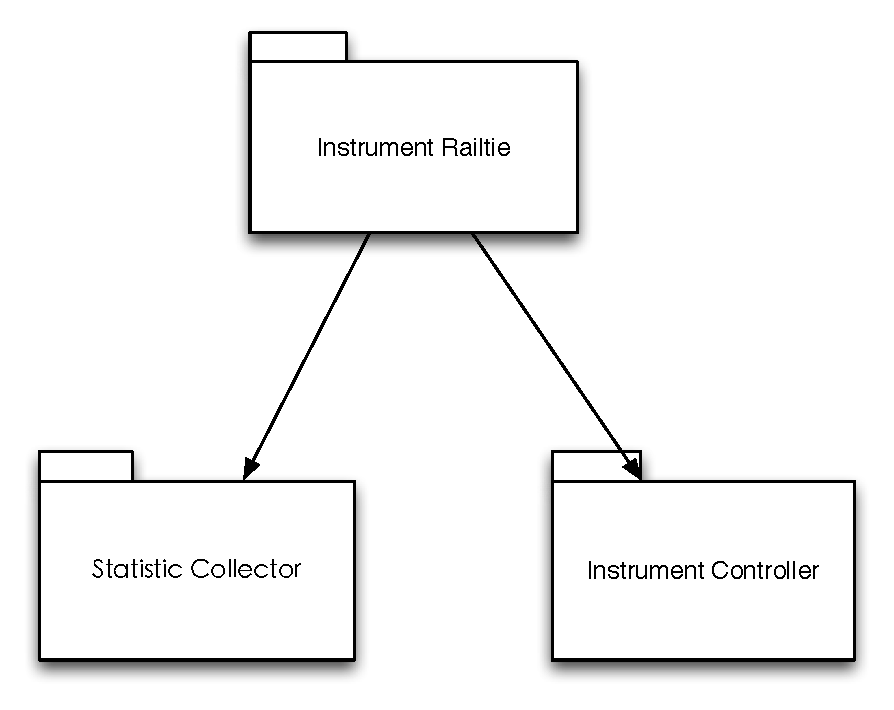
\includegraphics[width=0.7\textwidth]{images/overview/instrument_struct.eps}
\caption{Backend Instrumentation模块逻辑结构图}
\label{fig-instrument-struct}
\end{figure}

不难看到,Backend Instrumentation模块主要是由三个部分构成的,这三个部分的作用分别如是:Instrument Railtie是一个Railtie实例,它作为一个Railtie,使得整个Backend Instrumentation模块能够作为Rails的插件形式被载入和初始化。在初始化时,该模块负责判断当前环境,如果发觉是服务器环境,则载入相应代码逻辑并初始化其状态,若发觉是控制台环境,则避免载入代码逻辑;Statistic Collector则是负责实时收集Rails服务器端的性能数据(包括CPU占用率和内存使用率等),并将这些数据发送给前端浏览器;Backend Instrumentation Controller则是负责发送性能数据的接口,它是负责Rails服务器和浏览器客户端通信的总接口,浏览器通过该模块接收SSE消息,服务器通过该模块发送相应性能实时数据。

在Rails工程初始化时,Instrument Railtie首先将自己注册到Gemfile里,则会在其后被Rails自动载入,并调用其初始化接口进行初始化工作。Instrument Railtie初始化的第一步是判断自己是否运行在Rails服务器中,只有运行在服务器模式下,Instrument Railtie方才会载入Backend Instrumentation模块的其他组件,并进行相应的初始化工作。当Instrument Railtie完成初始化后,整个Backend Instrumentation系统便宣告正常工作。这时候Statistic Collector将开始收集服务器性能数据,按照预先设定好的采样时间(1秒),Statistic Collector将会对服务器主机的性能参数进行评估。Statistic Collector完成评估后会生成代表评估结果的性能参数,然后便会通过DRb告知服务器传送这一数据,DRb则会通知SSE模块将这一消息传递给浏览器客户端。这之后,Instrument Controller作为与浏览器客户端通信的代表,将会将这一消息序列化为字节流,并且实时地传递给前端浏览器。至此,浏览器便接收到来自于后端的实时性能数据,并作对这些数据加以利用(比如基于网页的管理终端显示实时图表等)。



\section{系统物理结构设计}
为了更加清楚地展示整个系统运行时的物理结构,图\ref{fig-physic}展示了整体结构:

\begin{figure}[h]
\centering
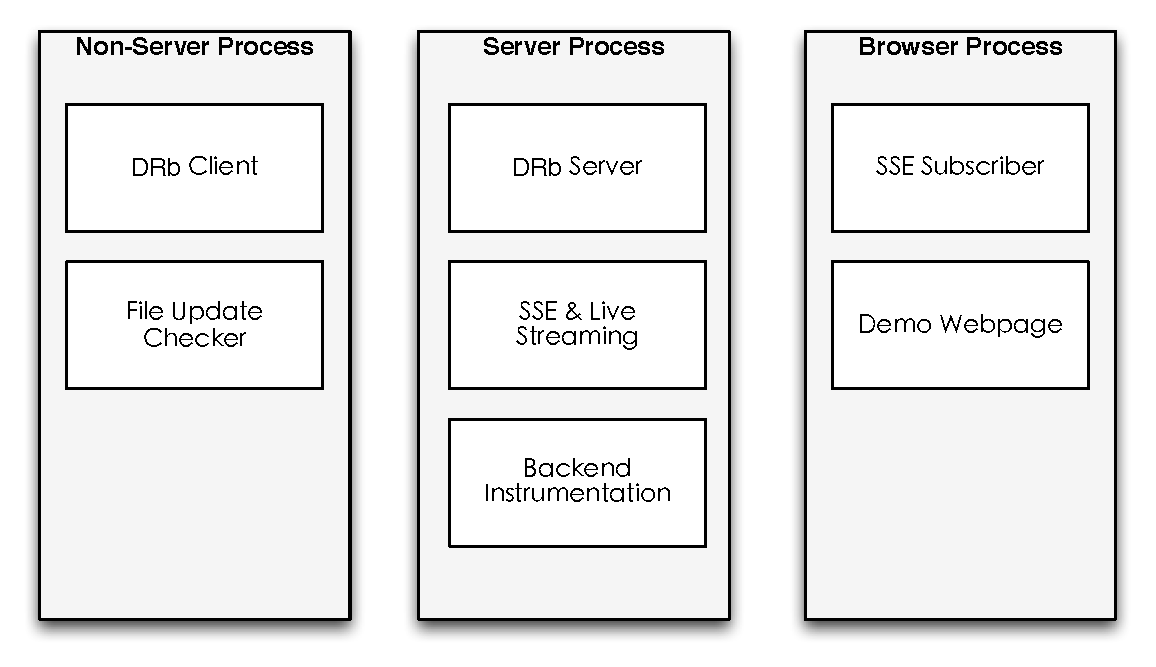
\includegraphics[width=0.7\textwidth]{images/overview/physic_logic.eps}
\caption{系统整体物理结构示意图}
\label{fig-physic}
\end{figure}

首先整个系统总体上是在三大物理运行实体中运行的,其中浏览器这一边是指用户使用的主机浏览器,本系统负责订阅SSE消息的模块驻留在该物理主机上,并且本项目开发的示例网页同样运行在该主机上。在服务器后端,本系统区分了服务器进程和非服务器进程,服务器进程往往将后台工作交予非服务器进程执行,但后者却难以同浏览器通信,这是区分这两个物理实体的原因。在本系统中,非服务器进程配备DRb客户端代码负责和服务器进程进行跨进程通信,并且本系统的文件系统监视模块驻留在非服务器进程之中。对于服务器进程,首先DRb服务器运行于其上,作为响应非服务器进程的模块,它负责在本地执行委托任务。另外的SSE和Live Streaming模块则是负责想浏览器传送实时数据和SSE消息,Backend Instrumentation负责收集实时性能数据,他们都是驻留在服务器进程中。










